\section{Results}\label{sec:results}


Figure \ref{fig:error-true-pop} examines how the hypothetical distributions proposed in Figure \ref{fig:dif-priv} appear in practice. The upper pane gives the distribution of population counts by racial category---the typical population counts within a census block group for people of color are significantly lower than those for white people. The lower pane, then, shows how a color-blind algorithm can have such a racialized effect. While the algorithms are not sensitive to whether they are estimating population counts for people of color or white people, they perform much worse (in that the absolute magnitude of percent error is much greater) when estimating smaller population counts, which are much more likely to belong to populations of color than to white populations.

\begin{figure}
   \centering
   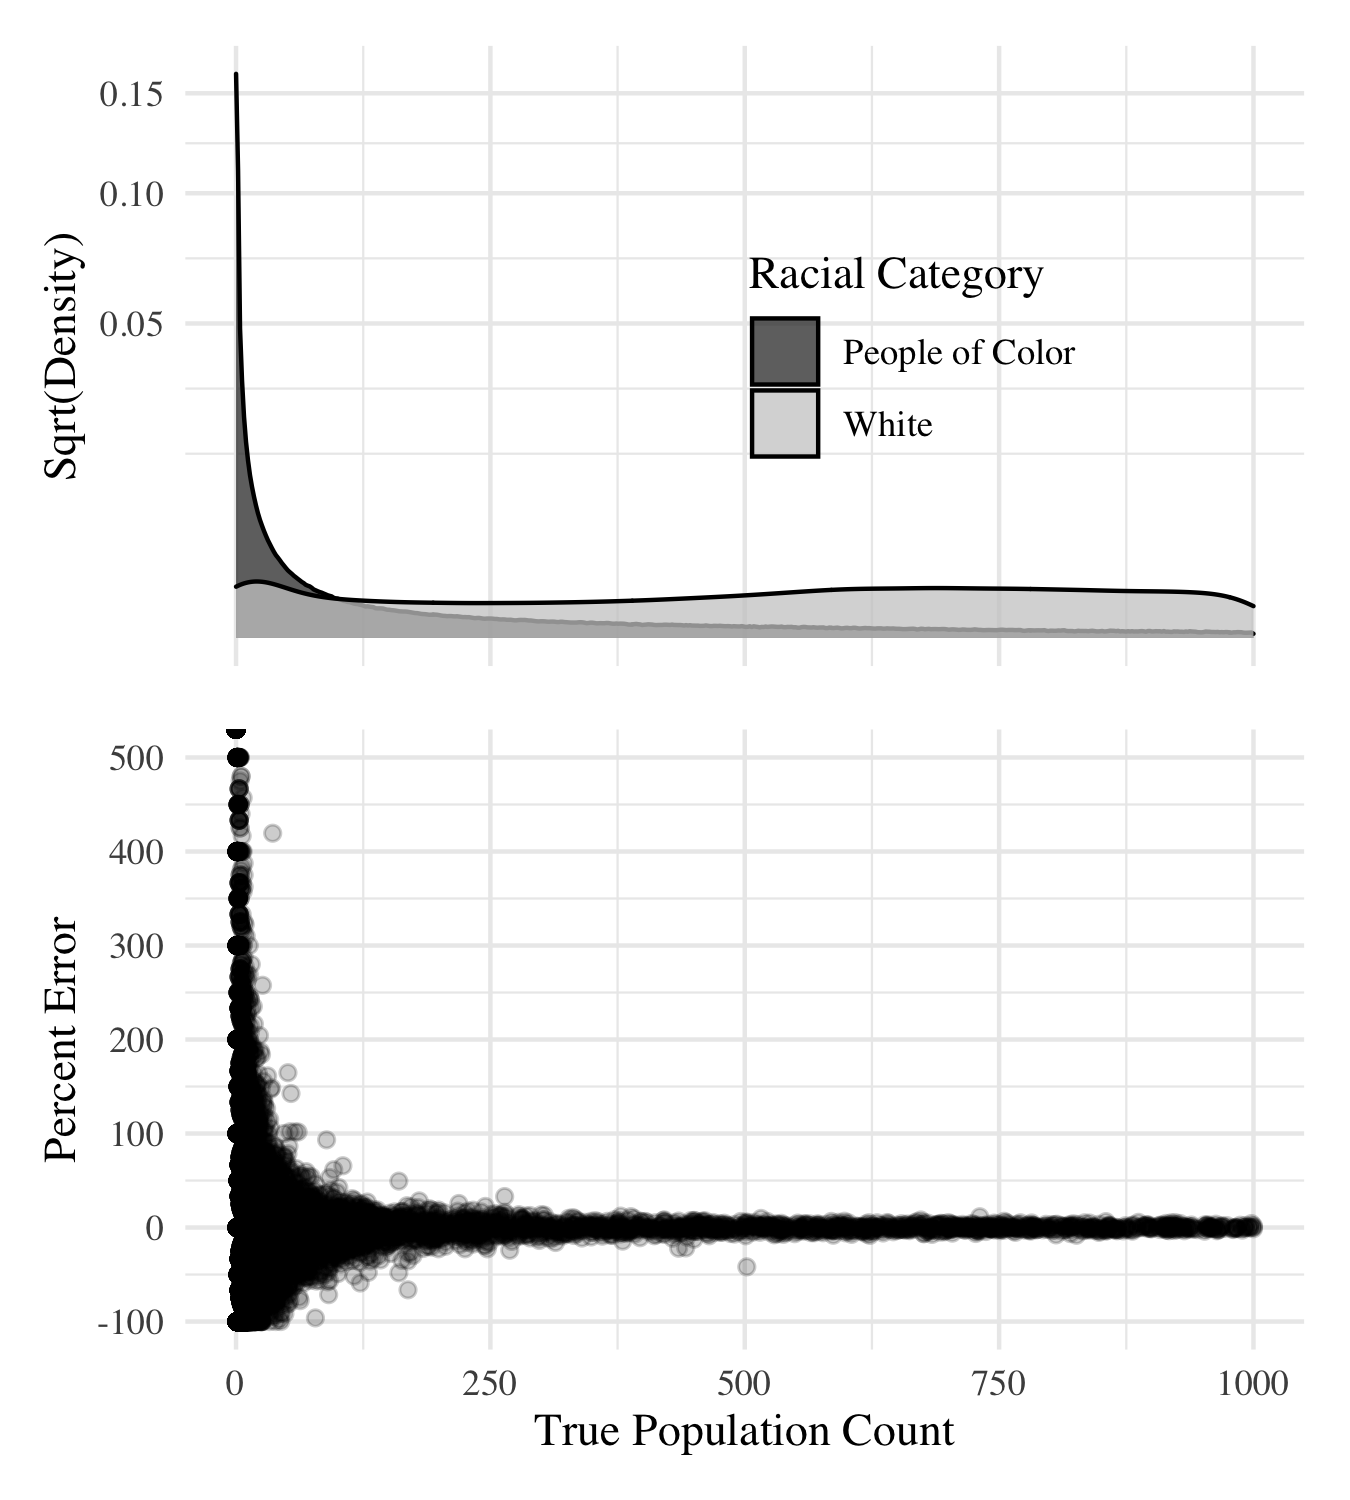
\includegraphics[width=0.75\textwidth]{figures/error_by_true_pop.png}
   \caption{A pair of plots showing the distribution of true population counts by census block group from the 2010 U.S. census, where the upper pane delineates the density by racial category, and the lower shows the distribution of percent error between true population count and differentially private estimate. Lower population counts are both more likely to occur when describing populations of color and more susceptible to significant error in estimation.}
   \label{fig:error-true-pop}
\end{figure}

Figure \ref{fig:error-by-race}, then, shows the implications of implementing differentially private algorithms in a use case such as that shown in Figure \ref{fig:error-true-pop}. In the trial run on 2010 Census data, the distributions of percent error have substantially greater variances for populations of color than for white populations. Further, too, the only distribution of percent error centered around zero is that of white populations; roughly in accordance with the absolute population size, the distribution of percent error is centered closer and closer to $-100$\% (complete erasure.) The Native Hawaiian and Pacific Islander categorization shows a particularly egregious example of this effect, with over 50\% of nonzero population counts completely erased. The fact that some of these distributions are centered around nonzero numbers should be puzzling to those familiar with differentially private algorithms, and is likely a result of post-processing and adjusting for invariants carried out by the Bureau.

\begin{figure}
   \centering
   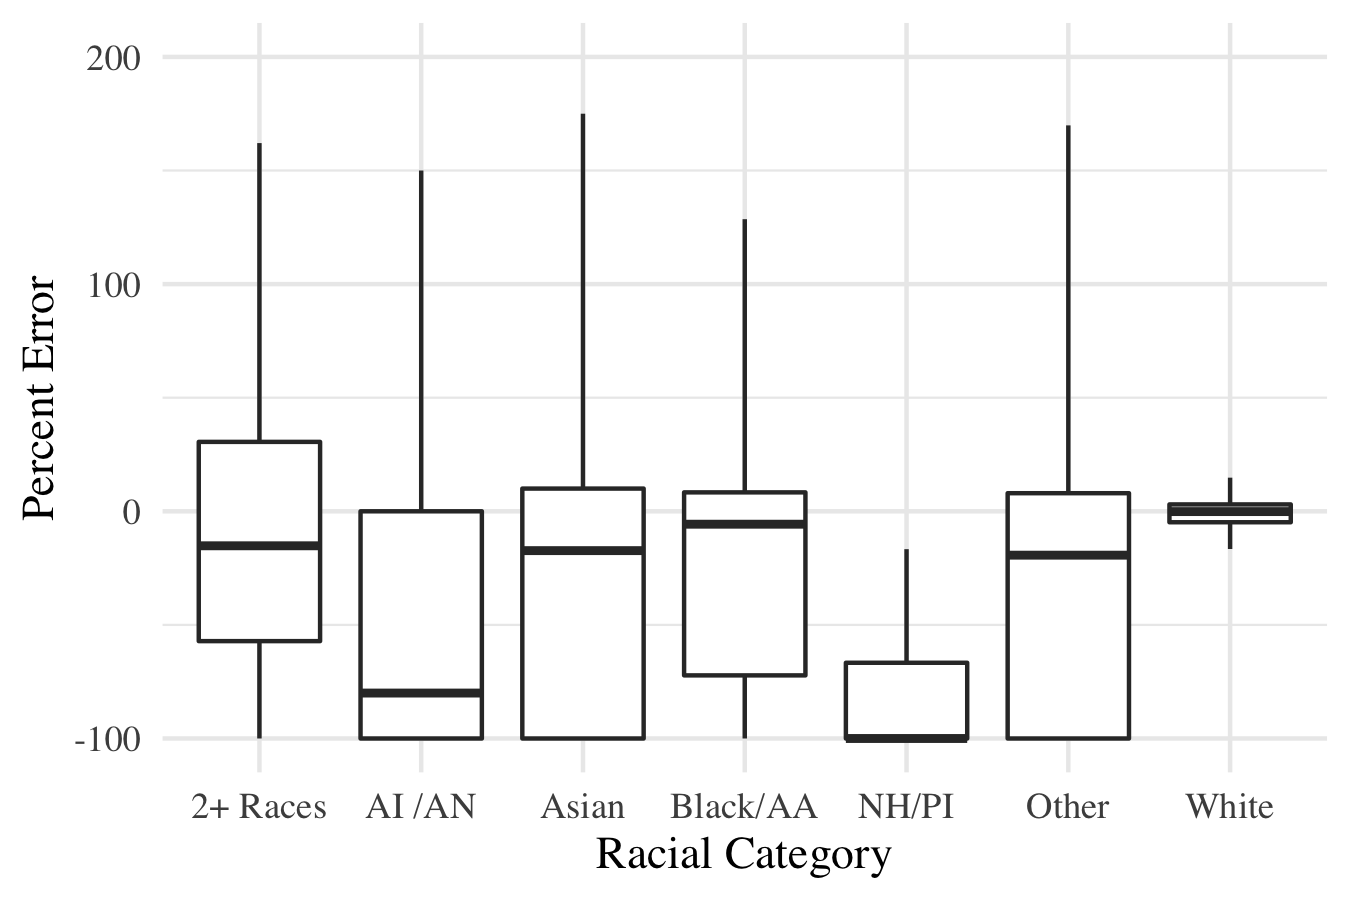
\includegraphics[width=0.75\textwidth]{figures/error_by_race.png}
   \caption{Distributions of percent error in estimation of true census block group population count by racial category. White populations experience, by far, the least deviation between true and estimated population counts, as well as the only distribution of percent error centered around zero.}
   \label{fig:error-by-race}
\end{figure}
 
\subsection{Erasing Races}\label{sec:erase}

Table \ref{tab:error-by} gives the proportion of estimates, by ethnoracial group, that experience abitrarily selected severities of error. Initially, consider the \textit{Population Erased} column, giving the proportion of nonzero populations estimated to contain zero people. For one, more generally, the proportion of populations erased by these algorithms is much greater for racial groups that identify as Hispanic/Latino than for those who do not. As before, smaller populations are increasingly subsceptible to this error; populations of people categorized as Hispanic/Latino Native Hawaiians or Pacific Islanders are erased in over 84\% of trials, and \textit{half} of the ethnoracial population subgroups are erased in at least 37\% of trials. By contrast, white populations are erased in less than 1\% of trials.

Similar disparities in estimation accuracy occur in the remaining three columns. While populations of color are also more likely to have their population counts drastically \textit{over}estimated, I contend that this is not cause for relief. The noise added to a statistic in the privatization process is completely independent of trial. That is, the previous perturbation of a population's true count has no bearing on the next. Resultantly, this overestimation is likely a `one-time' occurence, and, by the appearance of the distributions shown in Table \ref{tab:error-by}, is particularly vulnerable to complete erasure in the next census. As a result, drastic overestimation is also not an acceptable form of error, as it is simply an indicator of  instability.

% latex table generated in R 3.6.3 by xtable 1.8-4 package
% Mon May  4 10:50:06 2020
\begin{table}[ht]
\centering
\begin{tabular}{l|rrrr} 
 Ethnicity/Race Category & \multicolumn{4}{c}{Proportion of Estimates Resulting in Given Degree of Error} \\
 \hline
 & \thead{Population \\ Erased} & \thead{Less Than Half of \\ the True Population} & \thead{Twice the True \\ Population} & \thead{Ten Times the \\ True Population} \\ 
  \hline
H/L: 2+ Races & 0.179 & 0.179 & 0.107 & 0.014 \\ 
H/L: AI /AN & 0.469 & 0.469 & 0.087 & 0.009 \\ 
  H/L: Asian & 0.663 & 0.663 & 0.069 & 0.007 \\ 
  H/L: Black/AA & 0.379 & 0.379 & 0.088 & 0.009 \\ 
  H/L: NH/PI & 0.841 & 0.841 & 0.033 & 0.004 \\ 
  H/L: Other & 0.115 & 0.115 & 0.061 & 0.007 \\ 
  H/L: White & 0.055 & 0.055 & 0.029 & 0.002 \\ 
   \hline
Non-H/L: 2+ Races & 0.044 & 0.044 & 0.064 & 0.006 \\ 
  Non-H/L: AI /AN & 0.407 & 0.407 & 0.095 & 0.009 \\ 
  Non-H/L: Asian & 0.132 & 0.132 & 0.068 & 0.007 \\ 
  Non-H/L: Black/AA & 0.089 & 0.089 & 0.041 & 0.004 \\ 
  Non-H/L: NH/PI & 0.612 & 0.612 & 0.072 & 0.007 \\ 
  Non-H/L: Other & 0.529 & 0.529 & 0.094 & 0.009 \\ 
  Non-H/L: White & 0.006 & 0.006 & 0.005 & 0.000 \\ 
  \end{tabular}
  \caption{Proportion of estimates, by census ethnicity/race category, that result in selected degrees of estimation error. White, non-Hispanic/Latino populations are consistently well over an order of magnitude less likely to have their population erased by the differentially private algorithm than other ethnoracial categories. In general, the variability in differentially private population count estimates for populations of color is significantly greater than that for white populations.}
  \label{tab:error-by}
\end{table}

\subsection{Creating Races}\label{sec:create}

Another possible outcome resulting from the implementation of these algorithms is the estimation of positive subpopulation counts for subpopulations that do not exist. Table \ref{tab:nonzero-by} gives the proportion of cases in which this form of error occurs by ethnoracial category. Similarly to Table \ref{tab:error-by}, subpopulations are increasingly vulnerable to this form of inaccuracy as the true subpopulation size decreases.

% latex table generated in R 3.6.3 by xtable 1.8-4 package
% Mon May  4 10:50:08 2020
\begin{table}[ht]
\centering
\begin{tabular}{l|r}
 Ethnicity/Race Category & \thead{\% Estimated \\ Nonzero Count} \\ 
  \hline
  H/L: 2+ Races & 0.081 \\ 
  H/L: AI /AN & 0.171 \\ 
  H/L: Asian & 0.212 \\ 
  H/L: Black/AA & 0.135 \\ 
  H/L: NH/PI & 0.337 \\ 
  H/L: Other & 0.039 \\ 
  H/L: White & 0.012 \\ 
   \hline
  Non-H/L: 2+ Races & 0.009 \\ 
  Non-H/L: AI /AN & 0.064 \\ 
  Non-H/L: Asian & 0.042 \\ 
  Non-H/L: Black/AA & 0.018 \\ 
  Non-H/L: NH/PI & 0.206 \\ 
  Non-H/L: Other & 0.149 \\ 
  Non-H/L: White & 0.001 \\ 
  \end{tabular}
  \caption{Proportion of nonexistent populations that were estimated to have some nonzero population count by the differentially private estimators. White, non-hispanic/latino populations are at least an order of magnitude less likely to experience this misestimation than those in other ethnoracial categories.}
  \label{tab:nonzero-by}
\end{table}
















